\chapter{Case Of Study 1: Work-Stealing}

\section{Introduction}

It is known that any algorithm for some concurrent objects must use costly synchronization mechanisms, which might jeopardize performance. Thus, objects with relaxed semantics have been proposed to find algorithms devoid of such costly mechanisms. In this chapter, we explore whether there are non-trivial and useful relaxed objects that can be implemented using only synchronization mechanisms that are among the simplest ones without compromising performance.  We concretely focus on the case of work-stealing.

\subsection{Context}

\emph{Work-stealing} is a popular technique to implement dynamic \emph{load balancing} for efficient task parallelization of irregular workloads. It has been used in several contexts, e.g., programming languages, parallel-programming frameworks, SAT solvers and state-space exploration in model checking (e.g.~\cite{DBLP_journals_tpds_AyguadeCDHLMTUZ09, DBLP_journals_jpdc_BlumofeJKLRZ96, CGSDKEPS05, DBLP_conf_jvm_FloodDSZ01, DBLP_conf_pldi_FrigoLR98, DBLP_conf_java_Lea00, DBLP_conf_hpca_RangerRPBK07}).

In work-stealing, each process \emph{owns} a set of tasks that must be executed.  The \emph{owner} of the set can put tasks in it and can take tasks from it to execute them. When a process runs out of tasks (i.e., the set is empty), it becomes a \emph{thief} to steal tasks from a \emph{victim}. A work-stealing algorithm provides three high-level operations: \Put and \Take, which can be invoked only by the owner, and \Steal, which a thief can invoke. \emph{Linearizability}~\cite{DBLP_journals_toplas_HerlihyW90} is the usual assumed correctness condition, while \emph{nonblockingness}~\cite{DBLP_journals_toplas_HerlihyW90} and the stronger \emph{wait-freedom}~\cite{DBLP_conf_spaa_Herlihy91} are the typical  progress conditions.

A main target when designing work-stealing algorithms is to have \Put and \Take operations as simple and efficient as possible, as typically, they are the operations most intensively used by the owner. Unfortunately, it has been formally shown that any work-stealing algorithm in the standard asynchronous shared memory model must use \RAW synchronization patterns or atomic \RMW instructions (e.g., \CAS or \TAS)~\cite{DBLP_journals_jacm_AttiyaGHK09}. \RAW is a useful synchronization pattern based on the \emph{flag principle}, i.e., writing on a shared variable and then reading another variable (see~\cite {DBLP_books_daglib_0020056}). To correctly implement an algorithm using such a synchronization pattern in real multi-core architectures, a memory \emph{fence} (also called \emph{barrier}) needs to be explicitly added so that the \R and \W instructions are not reordered by the compiler or the architecture.  It is well-known that fences that avoid reads and writes to be reordered are highly costly, while atomic \RMW instructions, with high coordination power (which can be formally measured through the \emph{consensus number} formalism~\cite{DBLP_journals_toplas_Herlihy91}), are in principle slower than the simple \R/\W instructions.\footnote{In practice, contention might be the dominant factor, namely, an uncontended \RMW instruction can be faster than contended \R/\W instructions.} Indeed, the known work-stealing algorithms in the literature are based on the flag principle in their \Take/\Steal operations~\cite{circular.work.stealing, FLR98, non.blocking.work.stealing, 10.1145.571825.571876}.  Two possible ways to circumvent the impossibility result in~\cite{DBLP_journals_jacm_AttiyaGHK09} are to consider work-stealing with relaxed semantics or to make extra assumptions on the model.  As far as we know,~\cite{maged.vechev.2009} and~\cite{fencefreework} are the only works that follow these directions.

Observing that in some contexts, it is ensured that no task is repeated (e.g., by checking first if a task is completed) or the nature of the problem solved tolerates repeatable work (e.g., parallel SAT solvers), Michael, Vechev, and Saraswat propose \emph{idempotent} work-stealing~\cite{maged.vechev.2009}, a relaxation allowing a task to be taken \emph{at least once}, instead of \emph{exactly once}.  Three idempotent work-stealing algorithms are presented in~\cite{maged.vechev.2009}, where tasks are inserted/extracted in different orders.  The relaxation allows each of the algorithms to circumvent the impossibility result in~\cite{DBLP_journals_jacm_AttiyaGHK09} in its \Put and \Take operations as they use only \R/\W instructions and are devoid of \RAW synchronization patterns. However, \Steal uses \CAS. Moreover, \Put requires that some \W instructions are not reordered, and \Steal requires that some \R instructions are not reordered either, and thus fences are required when the algorithms are implemented. However, fences between \R (resp. \W) instructions are usually not too costly in practice. As for progress guarantees, \Put and \Take are wait-free while \Steal is only nonblocking.

Morrison and Afek consider the TSO model~\cite{DBLP_journals_cacm_SewellSONM10} and present two work-stealing algorithms in~\cite{fencefreework} whose \Put operation is wait-free and uses only \R/\W instructions,  and \Take and \Steal are either nonblocking and use \CAS, or blocking and use a \emph{lock}.  The algorithms are non-trivial adaptations of the well-known Cilk THE and Chase-Lev work-stealing algorithms~\cite{circular.work.stealing, FLR98} to the TSO model.  Generally speaking, in this model, \W (resp. \R) instructions cannot be reordered; hence, fences among \W (resp. \R) instructions are unnecessary. Additionally, each process has a local buffer where its \W instructions are stored until they are eventually propagated to the main memory (in FIFO order).  Reordering some \W (resp. \R) instructions of Morrison and Afek's algorithms compromises correctness. However, TSO prevents this from happening.  To avoid \RAW patterns, they assume bounded size \W buffers.

\section{\label{sec-ws-mult}Work-Stealing with Multiplicity}

Work-stealing with \emph{multiplicity} is a relaxation in which, roughly speaking, every task is extracted \emph{at least once}. If several operations extract it, they must be \emph{concurrent}.
In the formal set-sequential specification below (and in its variant in the next section), tasks are inserted/extracted in FIFO order. The definition can be easily adapted to encompass other orders (e.g., LIFO). Figure~\ref{fig-example-execution} depicts an example of a set-sequential execution of the work stealing with multiplicity, where concurrent \Take/\Steal operations can extract the same task.

\begin{figure}[ht]
  \begin{center}
    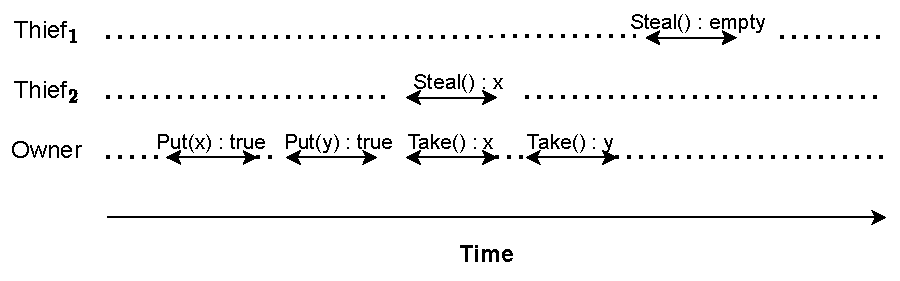
\includegraphics[width=0.95\textwidth]{contents/figures/IV_1_set-linearizability.pdf}
    \caption{\label{fig-example-execution}A set-sequential execution
      of work-stealing with multiplicity.}
  \end{center}
\end{figure}

\begin{definition}[FIFO Work-Stealing with Multiplicity\label{def-ws-mult}]

The universe of tasks that the owner can put in is \(\mathbf{N} = \{ 1, 2, \hdots \}\), and the set of states \(Q\) is the infinite set of finite strings \(\mathbf{N}^*\). The initial state is the empty string, denoted \(\epsilon\).  In state \(q\), the first element in \(q\) represents the \emph{head} and the last one the \emph{tail}. The transitions are the following:

{\def\OldComma{,}
 \catcode`\,=13
 \def,{%
   \ifmmode%
     \OldComma\discretionary{}{}{}%
   \else%
     \OldComma%
   \fi%
}%
\begin{enumerate}

\item \(\forall q \in Q\),
      \( \delta(q, \Put(x)) = (q \cdot x, \langle \Put(x): \true
      \rangle)\).

\item \(\forall q \in Q, 0\leq t\leq n-1\), \(x \in \mathbf{N}\), \(
      \delta(x \cdot q, \{\Take(), \Steal_1(), \hdots, \Steal_t() \})
      = (q, \{ \langle \Take():x \rangle, \langle \Steal_1():x \rangle,
      \hdots, \langle \Steal_t():x \rangle \})\).

\item \(\forall q \in Q\), \(1\leq t\leq n-1\), \(x \in \mathbf{N}\),
      \(\delta(x \cdot q, \{\Steal_1(), \hdots, \Steal_t() \}) =
      (q, \{\langle \Steal_1():x \rangle, \hdots, \langle
      \Steal_t():x \rangle\})\).

\item \(\delta(\epsilon, \Take()) = (\epsilon, \langle \Take(): \epty
      \rangle)\).

\item \(\delta(\epsilon, \Steal()) = (\epsilon, \langle \Steal(): \epty
      \rangle)\).

\end{enumerate}}

\end{definition}

Let \(\mathcal A\) be a set-linearizable algorithm for work-stealing with multiplicity.  Note that items 2 and 3 in Definition~\ref{def-ws-mult} and the definition of set-linearizability directly imply that in every execution of \(\mathcal A\), the number of \Take/\Steal operations that take the same task is, at most, the number of processes in the system, as the operations must be pairwise concurrent to be set-linearized together. Furthermore, every \emph{sequential} execution of \(\mathcal A\) (i.e., an execution where operations do not overlap in time) looks like an ``exact'' solution for work-stealing, as every operation is linearized alone, by definition of set-linearizability. Formally, every sequential execution of \(\mathcal A\) is a sequential execution of (FIFO) work-stealing. We call this property \emph{sequentially-exact}.  Thus, without contention, \(\mathcal A\) provides an exact solution for (FIFO) work-stealing.


\begin{remark}~\label{remark-seq-exact-set-lin}
Every set-linearizable algorithm for work-stealing with multiplicity is sequentially-exact.
\end{remark}

\subsection{\label{sec-ws-mult-max-reg}Work-Stealing with Multiplicity from \MaxReg}


Here, we show that work-stealing with multiplicity can be reduced to a single instance of a \MaxReg object (defined below).  Together with any of the fully \R/\W wait-free linearizable algorithms for \MaxReg in the literature, our algorithm provides a full \R/\W algorithm for work-stealing with multiplicity.  We will argue that using the \MaxReg algorithm in~\cite{DBLP_journals_jacm_AspnesAC12}, the resulting work-stealing algorithm with multiplicity has logarithmic step complexity and does not use \RAW synchronization patterns. The algorithm presented in this section does not seem to have practical implications. However, it will lead us to our efficient, fully fence-free \R/\W work-stealing algorithm with constant step complexity in all its operations.

Figure~\ref{figure-max-reg-mult} contains \WFWSM, a set-linearizable algorithm for work-stealing with multiplicity. The algorithm uses an atomic base object \MaxReg, which provides two operations: \MaxR returns the maximum value written so far in the object, and \MaxW writes a new value only if it is greater than the largest value written so far.


In \WFWSM, the tail of the queue is stored in the owner's local persistent variable \(tail\), while the head is stored in the shared \MaxReg \(Head\).  When the owner wants to put a new task, it first locally increments \(tail\) (Line~\ref{A01}) and then stores the task in the corresponding entry of \(Tasks\) and marks one more entry with \(\bot\) (Line~\ref{A02}); \(\bot\) indicates lack of tasks.  Recall that the notation in Line~\ref{A02} (instructions between brackets) denotes that the instructions can be executed in any order.  When the owner wants to take a task, it first reads the current head of the queue from \(Head\) (Line~\ref{A04}). Then, if there are tasks available (i.e., the head is less or equal to the tail), it reads the task at the head, updates \(Head\), and finally returns the task (Lines~\ref{A06} and~\ref{A09}); if there are no tasks available, the owner returns $\epty$ (Lines~\ref{A11}).  When a thief wants to steal a task, it first reads the current value of \(Head\) (Line~\ref{A12}) and then reads that entry of \(Tasks\) (Line~\ref{A13}).  If it reads a task (i.e. a non-\(\bot\) value), it updates \(Head\) and then returns the task (Lines~\ref{A16} and~\ref{A17}).  Otherwise, all tasks have been extracted, and it returns \epty (Line~\ref{A19}).

The semantics of \MaxW guarantees that $Head$ contains the current value of the head of the queue at all times, as a ``slow'' process cannot ``move back'' the head by writing a smaller value in \(Head\) (in Lines~\ref{A06} or~\ref{A16}).  Thus, the \MaxReg \(Head\) acts as a sort of barrier in the algorithm.  The net effect of this is that the only way that two \Take/\Steal operations return the same task is because they are concurrent, reading the same value from \(Head\).

%==================================================================
\begin{figure}[ht]
  \centering

  %% Reducción: Reduce tamaño de fuente
  \fbox{\tiny
    \begin{minipage}[t]{150mm} \footnotesize
      \renewcommand{\baselinestretch}{2.5} \resetline
      \begin{tabbing} aaaa\=aa\=aa\=aa\=aa\=aa\=aa\=\kill %~\\

        {\bf Shared Variables:}\\
        \> \> \(Head\): atomic $\MaxReg$ object initialized to \(1\)\\
        \> \> \(Tasks[1, 2, \hdots]\): array of atomic $\R/\W$ objects
        with\\ \>\>\>\>\>\>\> the first two objects initialized to \(\bot\)\\

        {\bf Persistent Local Variables of the Owner:}\\
        \> \> \(tail \leftarrow 0\)\\ \\

        {\bf Operation} \(\Put(x)\): \\
        \line{A01} \> \> \(tail \leftarrow tail + 1\)\\
        \line{A02} \> \> \(\{Tasks[tail].\W(x),\ Task[tail + 2].\W(\bot)\}\)\\
        \line{A03} \> \> {\bf return } $\true$\\
        {\bf end} $\Put$ \\ \\

        {\bf Operation} \(\Take()\): \\
        \line{A04} \> \> \(head \leftarrow Head.\MaxR()\)\\
        \line{A05} \> \> {\bf if \(head \leq tail\) then}\\
        \line{A06} \> \> \> \(\{ x \leftarrow Tasks[head].\R(),
        Head.\MaxW(head+1)\}\)\\
        % \line{A07} \> \> $head \leftarrow head+1$\\
        % AC: Miguel ya habia observado que la sigueinte linea no es
        % necesaria. Yo no habia entendido
        % \line{A08} \> \> $Head.\MaxW(head)$\\
        \line{A09} \> \> \> {\bf return} \(x\)\\
        \line{A10} \> \> {\bf end if}\\
        \line{A11} \> \> {\bf return} $\epty$\\
        {\bf end} $\Take$ \\ \\


        {\bf Operation} \(\Steal()\): \\
        \line{A12} \> \> \(head \leftarrow Head.\MaxR()\)\\
        \line{A13} \> \> \(x \leftarrow Tasks[head].\R()\) \\
        \line{A14} \> \> {\bf if \(x \neq \bot\) then}\\
        % \line{A15}\>  \> \> $head \leftarrow head+1$\\
        \line{A16} \> \> \> \(Head.\MaxW(head+1)\)\\

        \line{A17} \> \> \> {\bf return} \(x\)\\
        \line{A18} \> \> {\bf end if}\\
        \line{A19} \> \> {\bf return} $\epty$\\
        {\bf end} $\Steal$

      \end{tabbing}
    \end{minipage}
  }
  \caption{\label{figure-max-reg-mult}\WFWSM: a \MaxReg-based
    set-linearizable algorithm for work-stealing with multiplicity.}
\end{figure}
% =================================================================

Note that if only the first object in \(Tasks\) is initialized to \(\bot\) (and hence \Put is modified accordingly), a thief may read a value from \(Tasks\) that has not been written by the owner: in an execution with a single \(\Put(x)\) operation, the steps in Line~\ref{A02} could be executed \(Tasks[1].\W(x)\) first and then \(Tasks[2].\W(\bot)\) with a sequence of two \Steal operations completing in between, hence the second operations reading $Tasks[2]$ which has not been written yet by the owner, which is a problem if \(Tasks[2]\) contains a value distinct from non-\(\bot\) value.


\begin{theorem}\label{theo-wf}
  \WFWSM (Figure~\ref{figure-max-reg-mult}) is a set-linearizable wait-free fence-free algorithm for work-stealing with multiplicity using atomic \R/\W objects and a single atomic \MaxReg object. Moreover, all operations have constant step complexity, and \Put is fully \R/\W.
\end{theorem}

\begin{proof}

The algorithm is wait-free as every operation requires a constant number of steps to terminate, hence having constant step complexity.  Observe that \Put uses only \R/\W.  Moreover, the algorithm does not require any specific ordering among its steps beyond what is implied by data dependence; therefore, it is fully fence-free.

Before proving that \WFWSM is set-linearizable, we first observe that at any time, the thieves read the range of \(Tasks\) that the owner has already initialized; more specifically, every \Steal operation reads from \(Tasks\) (in Line~\ref{A13}), a value that was written by the owner, either \(\bot\) or a task.

At any time during an execution, the range \(Tasks[Head, Head+1, \hdots, ]\) contains a (possibly empty) sequence of tasks followed by at least one \(\bot\) value, considering the entries in index-ascending order. The claim is true initially as the first two entries if \(Tasks\) are initialized to \(\bot\).  Every time the owner stores a new task, it initializes a new entry of \(Task\) to \(\bot\) (in Line~\ref{A02}); hence the claim holds at any time, as \(Head\) is incremented only if the owner or a thief reads that \(Tasks[Head]\) contains a non-\(\bot\) value (in Lines~\ref{A06} or~\ref{A16}).  Note that the order of the instructions in Line~\ref{A02} is irrelevant.

We now prove that \WFWSM is set-linearizable. Consider any finite execution \(E\) of it. Since we already argued that the algorithm is wait-free, there is a finite extension of \(E\) in which all its operations are completed and no new operations start.  Thus, we can assume that there are no pending operations in \(E\).

First, note that the semantics of \MaxW implies that no pair of non-concurrent \Take/\Steal operations returns the same task: if two operations are not concurrent, then the first one increments the value of \(Head\) (and this value can only increment), and hence the second cannot read the same tasks from \(Tasks\). Thus, we have:

\begin{remark}\label{remark-concurrency}
If a task is returned by more than one \Take/\Steal operation, these operations are pairwise concurrent.  Thus, the owner's two distinct \Take operations cannot return the same task.
\end{remark}


The main observation for the set-linearizability proof is that at any time during the execution, the state of the object is represented by the tasks in the range \(Tasks[Head, Head+1, \hdots ]\), i.e., the sequence of non-\(\bot\) values (in index-ascending order) that written by the owner in that range. The set-linearization \(\SetLin(E)\) of \(E\) is obtained as follows:

\begin{itemize}

\item Every \Put operation is set-linearized \emph{alone} (i.e., in a concurrency class containing only the operation) placed at its step corresponding to \(Tasks[tail].\W(x)\) in \(E\) (Line~\ref{A02}).

\item For every task that is returned by at least one \Take/\Steal operation, all these operations are set-linearized in the same concurrency class placed at the first step \(e\) in \(E\) that corresponds to \(Head.\MaxW(head+1)\) (either in Line~\ref{A06} or~\ref{A16}) among the steps of the operations.  Note that \(e\) occurs between the invocation and response of every operation in the concurrency class. Since the operations return the same task, all of them execute the \MaxR steps in Lines~\ref{A04} or~\ref{A12} before \(e\), and, by definition, \(e\) appears in \(E\) before any other operation executes its step corresponding to \(Head.\MaxW(head+1)\).  Observe that the order in which the instructions in Line~\ref{A06} are executed is irrelevant.

\item Every \Take operation returning \epty is set-linearized alone, placed at its step in \(E\) corresponding to\\2\(Head.\MaxR()\) (Line~\ref{A04}).

\item Every \Steal operation returning \epty is set-linearized alone, placed at its step in \(E\) corresponding to \(Head.\MaxR()\) (Line~\ref{A12}).

\end{itemize}

Every concurrency class of \(\SetLin(E)\) is placed at a step of \(E\) that lies between the invocation and response of each operation in the concurrency class, which immediately implies that \(\SetLin(E)\) respects the partial order \(<_E\) of~\(E\). Thus, to conclude that \(\SetLin(E)\) is a set-linearization of \(E\), we need to show that it is indeed a set-sequential execution of the work-stealing with multiplicity.

First, note that a task can be extracted by a \Take/\Steal operation only if the \Put operation that stores the task executes its step corresponding to \(Tasks[tail].\W(x)\) (in Line~\ref{A02}) before the \Take/\Steal operation reads the entry of \(Tasks\) where the task is stored.  Thus, in \(\SetLin(E)\), every task is inserted before it is extracted.

Now, \Put stores tasks in \(Tasks\) in index-ascending order.  Due to the semantics of \MaxReg, \(Head\) never ``moves back'', i.e., it only increments one by one, and hence \Take and \Steal extract tasks in index-ascending order too.  Tasks in \(\SetLin(E)\) are inserted/extracted in FIFO order.

More specifically, for any concurrency class \(C\) of \(\SetLin(E)\) with \Take/\Steal operations that return the same tasks~\(x\), right before the step \(e\) of \(E\) where \(C\) is set-linearized, we have that \(x\) is the task with smallest index (left-most) in the range \(Tasks[Head, Head+1, \hdots]\), and thus indeed the operations in \(C\) get the oldest task in the object.

It only remains to be argued that any \Take/\Steal operation that returns \epty, do so correctly, i.e., each of these operations is set-linearized at a step of \(E\) at which \(Tasks[Head, Head+1, \hdots]\) is empty, i.e., all its entries initialized by the owner in that range contain \(\bot\).

Consider any \Take operation in \(E\) that returns \(\epty\). Observe that this can happen only if the owner sees that \(head > tail\), namely, the conditional is not satisfied in Line~\ref{A05}.  This is possible only when no item has been inserted, or all items have been extracted, and hence \(Tasks[Head, Head+1, \hdots]\) is empty.  Consider any \Steal operation in \(E\) that returns \(\epty\).  This is possible only when the thief reads \(\bot\) from \(Tasks\) in Line~\ref{A13}, and since we already argued that the owner inserts tasks in ascending order, the sequence \(Tasks[Head, Head+1, \hdots]\) is empty.

We conclude that \(\SetLin(E)\) is a valid set-sequential execution of work-stealing with multiplicity, and as it respects the partial order \(<_E\) of \(E\), we have that it is a set-linearization of \(E\), and therefore \WFWSM is set-linearizable. The theorem follows.
\end{proof}

If we replace \(Head\) with the wait-free linearizable \R/\W\ \MaxReg algorithm in~\cite{DBLP_journals_jacm_AspnesAC12}, whose step complexity is \(O(\log m)\), where \(m \ge 1\) is the maximum value that can be stored in the object, the step complexity of \WFWSM is bounded wait-free with logarithmic step complexity too. In the resulting algorithm, at most $m$ tasks can be inserted.  Since the algorithm in~\cite{DBLP_journals_jacm_AspnesAC12} does not use \RAW synchronization patterns (as explained in the proof of Theorem~\ref{theo-wf-log}), the resulting algorithm does not use those patterns either.

\begin{theorem}\label{theo-wf-log}
If $Head$ is an instance of the wait-free linearizable \R/\W\ \MaxReg algorithm in~\cite{DBLP_journals_jacm_AspnesAC12}, \WFWSM is set-linearizable, fully \R/\W and \Take and \Steal have step complexity $O(\log m)$, where $m$ denotes the maximum number of tasks that can be inserted in an execution. Furthermore, \Take and \Steal do not use \RAW synchronization patterns.
\end{theorem}

\begin{proof}
The algorithm remains set-linearizable by composability of set-linearizability\\~\cite{DBLP_journals_jacm_CastanedaRR18}.  While the step complexity of \Put is $O(1)$, the step complexity of \Take and \Steal is $O(\log m)$ as the step complexity \MaxR and \MaxW of the \MaxReg algorithm in~\cite{DBLP_journals_jacm_AspnesAC12} is $O(\log m)$.

We now argue that \Take and \Steal do not use \RAW synchronization patterns.  The reason is that the \MaxReg algorithm in~\cite{DBLP_journals_jacm_AspnesAC12} does not use this synchronization mechanism.  Roughly speaking, the algorithm consists of a binary tree of height $O(\log m)$ with an atomic bit in each of its nodes.  When a process wants to perform \MaxR, it reads the bits in a path of the tree from the root to a leaf and then returns a value according to the leaf it reached; the next node in the path the process reads depends on the current node's value.  When a process wants to perform \MaxW, it reads the bits in a path from the root to a leaf, which is on function of the binary representation of the value the process wants to write; then, if the new value is larger than the current one, in a bottom-up manner, it writes 1 in every node in the path with 0 (for the algorithm to be linearizable, the writes should occur in this order).  Thus, we have that \MaxR consists of a sequence of reads, and \MaxW consists of a sequence of reads followed by a (possibly empty) sequence of writes.  Therefore, \Take/\Steal of \WFWSM consists of a sequence of reads followed by a (possibly empty) sequence of writes, and thus the operation does not use \RAW synchronization patterns.
\end{proof}